\chapter{Podstawy teoretyczne}

Pierwsza wzmianka o użyciu tęczówki w celu identyfikacji jednostki datowana jest na rok
1936, a autorem jej był okulista Frank Burch \cite{FBIGov}. W roku 1985 okuliści Leonard Flom oraz
Aran Safir przedstawili tezę popartą badaniami klinicznymi, że w świecie nie istnieją dwie
identyczne tęczówki, a w roku 1987 opatentowali pomysł Bruch'a. Nie byli oni jednak w
stanie stworzy\'c systemu i algorytmów pozwalających na identyfikację osoby na podstawie
obrazu tęczówki. W roku 1989, na ich prośbę, matematyk John Daugman stworzył algorytmy
pozwalające na automatyczną identyfikację tęczówki, które następnie opatentował w roku 1994.
\cite{Misztal2012}
Algorytmy te są podwaliną większości rozwiąza\'n zastosowanych w systemach wykorzystujących
obraz tęczówki oka. W dalszej części tego rozdziału przedstawione zostaną informacje teoretyczne
pozwalające na zrozumienie jaką rolę odgrywa rozpoznawanie tęczówki w systemach biometrycznych.

\section{Budowa tęczówki}

\begin{figure}[ht]
  \centering
  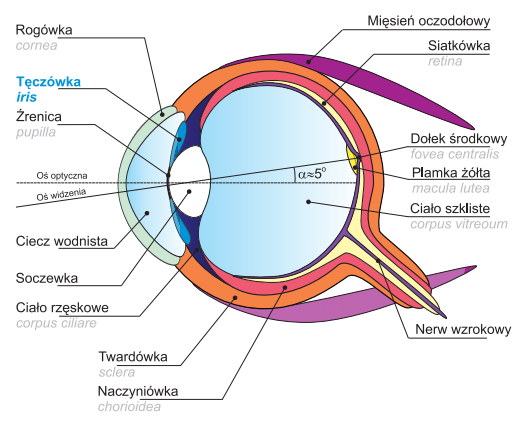
\includegraphics[width=0.7\textwidth]{images/intro/eyeStructure.png}
  \caption{Schemat anatomiczny oka ludzkiego \cite{Czajka}.}
  \label{fig:eyeStructure}
\end{figure}

Tęczówka jest umięśnioną częścią błony naczyniowej, która otacza otwór zwany \'zrenicą.
Jej częś\'c obwodowa przechodzi w ciało rzęskowe utrzymujące soczewkę \cite{Czajka}. Z zewnątrz
otoczona jest prze\'zroczystą rogówką pełniącą funkcję ochronną. Głównym zadaniem tęczówki
jest kontrolowanie strumienia światła dostającego się przez \'zrenicę do oka przez kurczenie i
rozkurczanie swoich mięśni. Bierze ona również udział w procesie akomodacji oka odpowiedzialnym
za ostre widzenie. Dzięki zawartemu w jej komórkach barwnikowi - \textit{melaninie}, może ona przyjmowa\'c różne kolory.
Kolor tęczówki najcześciej jest pomijany w procesie rozpoznawania ze względu na liczne możliwości
jego zaburzenia przykładowo w wyniku chorób lub zmian hormonalnych regulujących stężenie melaniny.

Patrząc na obraz tęczówki (rysunek \ref{fig:irisExample}) możemy dostrzec jej charakterystyczną teksturę. Wynika ona z ułożenia
beleczek i zatok na jej powierzchni. Tęczówka kształtuje się od trzeciego do ósmego miesiąca życia
płodowego i pozostaje niezmienna do końca życia (zakładając brak chorób).
W wyniku zgonu ulega zniszczeniu w ciągu pięciu sekund.

\begin{figure}[ht]
  \centering
  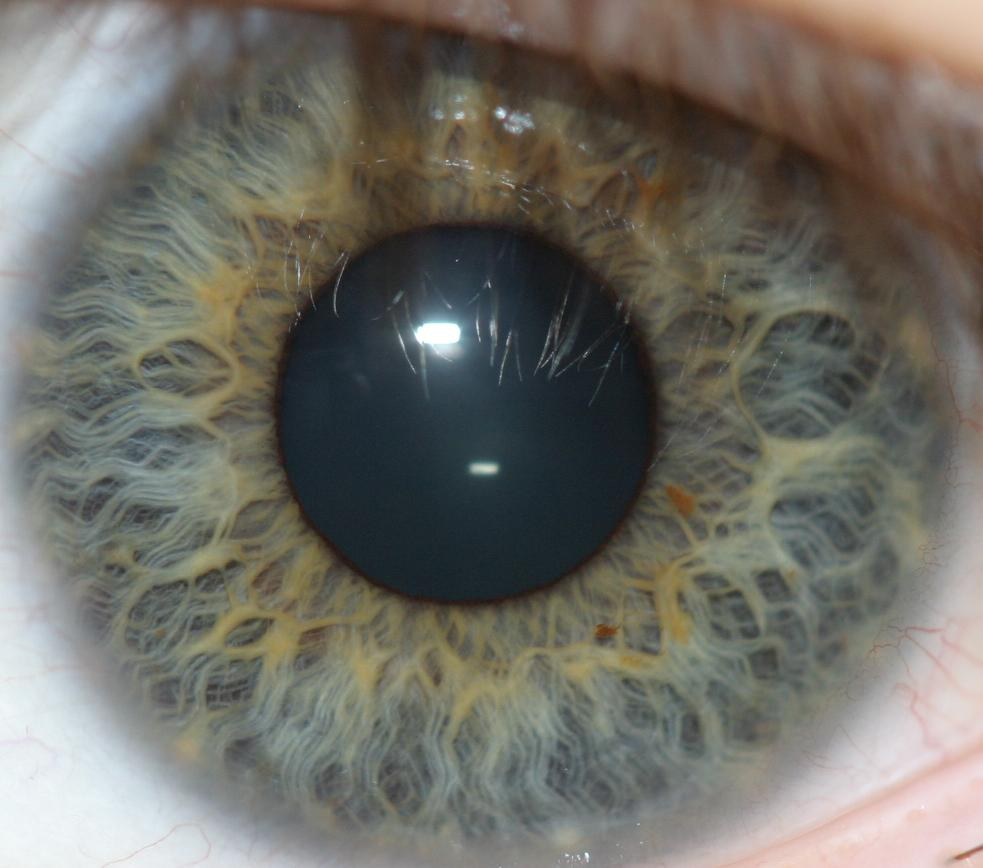
\includegraphics[width=0.5\textwidth]{images/intro/irisExample.png}
  \caption{Przykładowy obraz tęczówki oka.}
  \label{fig:irisExample}
\end{figure}

\section{Tęczówka w biomterii}

Aby cechy fizyczne były użyteczne z punktu widzenia biometrii powinny spełnia\'c następujące
wymagania:

\begin{itemize}
  \item uniwersalnoś\'c - każdy człowiek powinien posiada\'c daną cechę,
  \item unikalno\'c - cecha powinna by\'c unikalna dla każdej osoby,
  \item mierzalnoś\'c - łatwoś\'c pobrania informacji,
  \item trwałoś\'c i niezmiennoś\'c - cecha powinna by\'c niezmienna w trakcie życia,
  \item szybkoś\'c i skutecznoś\'c działania systemu opartego o cechę,
  \item akceptowalnoś\'c społeczna,
  \item niemożliwoś\'c podrobienia.
\end{itemize}

Tęczówka spełnia powyższe wymagania w stopniu bardzo dobrym. Większoś\'c populacji posiada
ją. Badania wykazują, że jest ona unikalna dla każdego człowieka, nawet dla bli\'zniąt jednojajowych.
Co więcej, tęczówki oka lewgo i prawego u jednego człowieka również różnią się między sobą. Tęczówka zawiera
wiele punktów charakterystycznych i detali, dzięki czemu rośnie skutecznoś\'c systemu opartego na jej obrazie.
Tak jak wcześniej zostało to wspomniane, tęczówka kształtuje się na etapie płodu i pozostaje niezmienna
przez resztę życia. Dzięki rozszerzaniu i kurczeniu się w celu kontrolowania przepływu światła w zależności
od oświetlenia otoczenia, oszukanie systemu przez zdjęcie jest mocno utrudnione. Dodatkowym atutem
jest fakt, że tęczówka jest dobrze chronionym, a jednocześnie dobrze widocznym organem, co ułatwia
pobranie obrazu.\newline

\noindent
Poniżej wymienione zostały wady tęczówki jako cechy biometrycznej:

\begin{itemize}
  \item jest stosunkowo mała, co znacznie zmniejsza dystans z jakiego można pobra\'c o niej informacje,
  \item znajduje się za wilgotną, zakrzywioną i odbijającą światło powierzchnią, co może potencjalnie
  wprowadza\'c zakłócenia w pobieranym obrazie,
  \item jest umiejscowiona na ruchomej gałce ocznej, która umiejscowiona jest na ruchomej głowie, co może
  wprowadza\'c liczne niespójności rotacji między obrazami tej samej tęczówki,
  \item częściowo zasłonięta przez powieki oraz rzęsy,
\end{itemize}

W tabeli poniżej (\ref{tab:irisBiometricsComparison}) przedstawione zostało porównanie tęczówki
z innymi cechami biometrycznymi w ramach wyżej wymienionych wymagań:

\begin{table}[h]
  \centering
  \begin{tabular}{|l|>{\centering}p{1cm}|>{\centering}p{1cm}|>{\centering}p{1cm}|>{\centering}p{1cm}|>{\centering}p{1cm}|>{\centering}p{1cm}|>{\centering}p{1cm}| }
    \hline
    \rowcolor{gray!20}
    Cecha biometryczna & \rotatebox{90}{Uniwersalnoś\'c} & \rotatebox{90}{Unikalnoś\'c} & \rotatebox{90}{Trwałoś\'c} & \rotatebox{90}{Mierzalnoś\'c} & \rotatebox{90}{skutecznoś\'c} & \rotatebox{90}{Akceptowalnoś\'c} \rotatebox{90}{społeczna} & \rotatebox{90}{Niemożliwoś\'c} \rotatebox{90}{podrobienia} \tabularnewline
    \hline\hline
    DNA & H & H & H & L & H & L & L \tabularnewline
    \hline
    Ucho & M & M & H & M & M & H & M \tabularnewline
    \hline
    Twarz & H & L & M & H & L & H & H \tabularnewline
    \hline
    Odciski palców & M & H & H & M & H & M & M \tabularnewline
    \hline
    Geometria dłoni & M & M & M & H & M & M & M \tabularnewline
    \hline
    Rozkład żył dłoni & M & M & M & M & M & M & L \tabularnewline
    \hline
    \rowcolor{yellow!50}
    Tęczówka & H & H & H & M & H & L & L \tabularnewline
    \hline
    Siatkówka & H & H & M & L & H & L & L \tabularnewline
    \hline
    Podpis & L & L & L & H & L & H & H \tabularnewline
    \hline
    Głos & M & L & L & M & L & H & H \tabularnewline
    \hline
  \end{tabular}
  \caption{Porównanie cech biometrycznych (na podstawie pozycji \cite{IntroToBiometricRecognition}). Legenda: H - spełnione w wysokim
  stopniu, M - spełnione w średnim stopniu, L - spełnione w niskim stopniu.}
  \label{tab:irisBiometricsComparison}
\end{table}

\section{Opis procesu rozpoznawania}

\noindent
Proces rozpoznawania tęczówki (rysunek \ref{fig:processDiagram}) można podzieli\'c na kilka etapów:

\begin{itemize}
  \item pobranie obrazu tęczówki,
  \item segmentacja,
  \item normalizacja,
  \item detekcja cech charakterystycznych
  \item dopasowanie
\end{itemize}

\begin{figure}[ht]
  \centering
  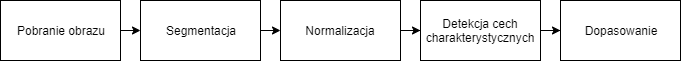
\includegraphics[width=0.8\textwidth]{images/intro/processDiagram.png}
  \caption{Diagram przedstawiający przebieg procesu rozpoznawania tęczówki}
  \label{fig:processDiagram}
\end{figure}

Pobranie obrazu tęczówki może wydawa\'c się stosunkowo proste, jednak zdecydowanie takie nie
jest. Zdjęcia tęczówki wykonywane w świetle widzialnym dają dobre wyniki dla tęczówek o jasnych
kolorach, natomiast podejście to może zawieś\'c w przypadku ciemnych kolorów tęczówek ze względu
na niski kontrast zdjęcia. Może to prowadzi\'c do zlania się \'zrenicy i tęczówki w jedną całoś\'c.
Uniemożliwiłoby to wyodrębnienie tych dwóch elementów w etapie segmentacji.

Pobieranie obrazu w świetle widzialnym może również prowadzi\'c do zmian szerokości tęczówki w trakcie
pobierania zdję\'c (różnica w oświetleniu między przetwarzaniem tęczówki w celu zapisania użytkownika
do bazy danych, a w momencie weryfikacji tożsamości), co może negatywnie wpływa\'c na działanie
systemu. Dodatkową wadą takiego podejścia jest występowanie w obrazie odbi\'c światła.

W celu wyeliminowania powyższych problemów zdjęcia tęczówki można wykonywa\'c w bliskiej podczerwieni \cite{IrisRecognitionPresentation},
dzięki czemu uzyskane obrazy nie posiadają zakłóceń w postaci odbi\'c światła, a także
zapewniają widocznoś\'c struktury tęczówki zarówno dla tych o jasnych, jak i ciemnych kolorach (rysunek \ref{fig:irisAcquisitionExample}).

\begin{figure}[ht]
  \centering
  \begin{subfigure}[b]{0.4\textwidth}
    \centering
    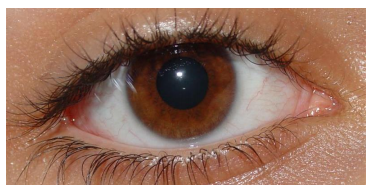
\includegraphics[width=\textwidth]{images/intro/eyeDaylight.png}
    \caption{Obraz tęczówki w świetle widzialnym}
  \end{subfigure}
  \begin{subfigure}[b]{0.4\textwidth}
    \centering
    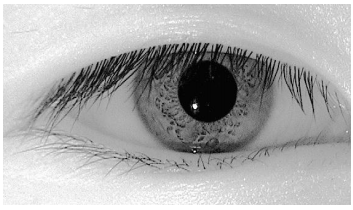
\includegraphics[width=\textwidth]{images/intro/eyeInfraRed.png}
    \caption{Obraz tęczówki w bliskiej podczerwieni}
  \end{subfigure}
  \caption{Róznice w pobieraniu obrazu tęczówki \cite{IrisRecognitionPresentation}.}
  \label{fig:irisAcquisitionExample}
\end{figure}


Następnie obraz poddawany jest procesowi segmentacji, którego zadaniem jest wydzielenie tęczówki z obrazu
całego oka. W tym celu określane są parametry okręgów
tęczówki oraz \'zrenicy takie jak ich punkty środkowe oraz promienie. Często w ramach segmentacji
wykonywane jest również poszukiwanie powiek oraz innych zakłóceń na obrazie np. rzęs. Piksele im odpowiadające
zapisywane są w masce zakłóceń określającej które fragmenty obrazu są znaczące dla procesu rozpoznawania,
a które nie. Algorytmy te działają w większości w oparciu o metody wykrywania krawędzi.
Metody segmentacji nie są przedmiotem niniejszej pracy i nie zostały w niej opisane.\newline

Znając parametry \'zrenicy oraz tęczówki możliwe jest wyodrębnienie z obrazu tylko i wyłącznie
punktów należących do tęczówki i zignorowanie reszty punktów obrazu. Wiedząc które piksele obrazu
reprezentują tęczówkę, możliwe jest przejście do kolejnego etapu, czyli ekstrakcji cech charakterystycznych
opisujących daną tęczówkę i zakodowania tych informacji w pewnej postaci. Dokonywane jest to w etapie kodowania
tęczówki. Posta\'c ta powinna umożliwia\'c porównanie dwóch reprezentacji tęczówek i podjęcie decyzji o dopasowaniu
bąd\'z niedopasowaniu.

Aby umożliwi\'c porównanie dwóch tęczówek należy zapewni\'c jednolity rozmiar
ich obrazów lub reprezentacji. W tym celu obrazy poddawane są procesowi normalizacji.

Tak jak wcześniej zostało wspomniane, pierwszym, pionierskim systemem rozpoznawania tęczówki był
system opracowany przez Johna Daugmana \cite{DaugmanHowIrisRecognitionWorks}. Nie jest to jednak
jedyna praca traktująca o rozpoznawaniu tęczówki. W swoich pracach alternatywne rozwiązania
zaproponowali również Wildes \cite{Wildes} oraz Boles \cite{Boles}. W następnym rozdziale opisane
zostały algorytmy autorstwa Daugmana oraz ich implementacje.

\section{Zastosowania}

Ze względu na dokładnoś\'c działania i koszty związane z wprowadzeniem tego typu systemu
biometrycznego, zastosowania rozpoznawania tęczówki można znale\'z\'c głównie w systemach
wymagających największego stopnia bezpieczeństwa.

Jednym z sektorów w którym rozpoznawanie tęczówki znajduje miejsce jest bankowoś\'c. Banki
przechowują wiele tajnych informacji, które przedstawiane są osobom tylko i wyłącznie
po wcześniejszej weryfikacji tożsamości. Potencjalne naruszenia bezpieczeństwa mogłyby doprowadzi\'c
do wycieku danych osobowych czy nawet kradzieży.

Rozpoznawanie tęczówki znajduje również zastosowanie w sektorze zdrowia. Pozwala ono na dokładną
identyfikację osoby i ustalenie statusu ubezpieczenia, a także prostsze odnalezienie kartoteki
medycznej. Znalazły one zastosowanie w szpitalach w całym świecie w celu rozwiązania problemu z
kradzieżami noworodków. Dostęp do sali w której znajduje się dziecko posiadają jedynie doktorzy,
pielęgniarki oraz matka dziecka.

Jednym z największych sektorów w których stosowane jest rozpoznawanie tęczówki jest kontrola graniczna
oraz imigracyjna. W wielu krajach postanowiono uży\'c wzoru tęczówki przechowywanego w systemie jako głównego
zabezpieczenia przed nielegalnym przekroczeniem granicy. Rozwiązania takie zostały zaimplementowane na lotniskach
w Stanach Zdjednoczonych, Kanadzie, Wielkiej Brytanii czy Holandii.

Jednym z największych zastosowań jest projekt Aadhaar w Indiach, którego celem było wprowadzenie
unikalnego identyfikatora tożsamości dla obywateli Indii. Zgodnie ze stroną zawierającą statystyki na
temat tego projektu (zasób \ref{web:aadhaar}), liczba wygenerowanych identyfikatorów wynosi 1 224 576 859.
Identyfikator ten bazowany jest na danych
osobistych oraz danych biometrycznych - między innymi wzorze tęczówki. Celem projektu jest zebranie
informacji, w tym wzorów tęczówki, wszystkich obywateli Indii \cite{DaugmanIndia}. Projekt powstał w
celu poprawy systemu przydzielania świadczeń socjalnych i innych programów pomocy przez redukcję oszustw.
Podobne programy mające na celu stworzenie krajowego identyfikatora zawierającego dane biometryczne
zostały rozpoczęte przez Indonezję oraz Singapur \cite{DaugmanApplications}.

